\chapter{Similariteit}

Een similariteitsmaat voor afbeeldingen is een maat die de gelijkenis tussen twee gegeven
afbeelding uitdrukt als een getal uit het interval $[0,1]$. Dit getal nadert naar 1
naarmate de gelijkenis groter is. Bijgevolg kunnen we een dergelijke maat gebruiken om
een lijst van zoekresultaten te herordenen volgens similariteit met een bepaalde 
voorbeeld-afbeelding uit die lijst. 

We construeren een similariteitsmaat voor afbeeldingen in twee stappen. Eerst identificeren we
een afbeelding, al dan niet rechtstreeks, met een (L-)vaagverzameling. Daarna maken we gebruik van
de vaagsimilariteitsmaten uit \ref{sectie:vaagsimilariteitsmaten} om deze (L-)vaagverzamelingen te
vergelijken. 

In het vervolg van deze scriptie bedoelen we met de term ``similariteitsmaat'' steeds
een similariteitsmaat voor afbeeldingen. Dit omvat dus zowel een manier van identificeren als een 
vaagsimilariteitsmaat.

\section{Evaluatie van performantie}

Om uit meerdere similariteitsmaten de meest geschikte te kiezen, 
moeten we een manier vinden om een dergelijke maat objectief te beoordelen. 
Dit zullen we doen door elke
maat, voor een bepaalde voorbeeld-afbeelding, toe te passen op een eenzelfde collectie 
van afbeeldingen. Vervolgens zullen we de rangschikking die we zo bekomen
beoordelen met behulp van een performantiemaat.


\begin{figure}[p]
\begin{center}
%\subfigure[]{
%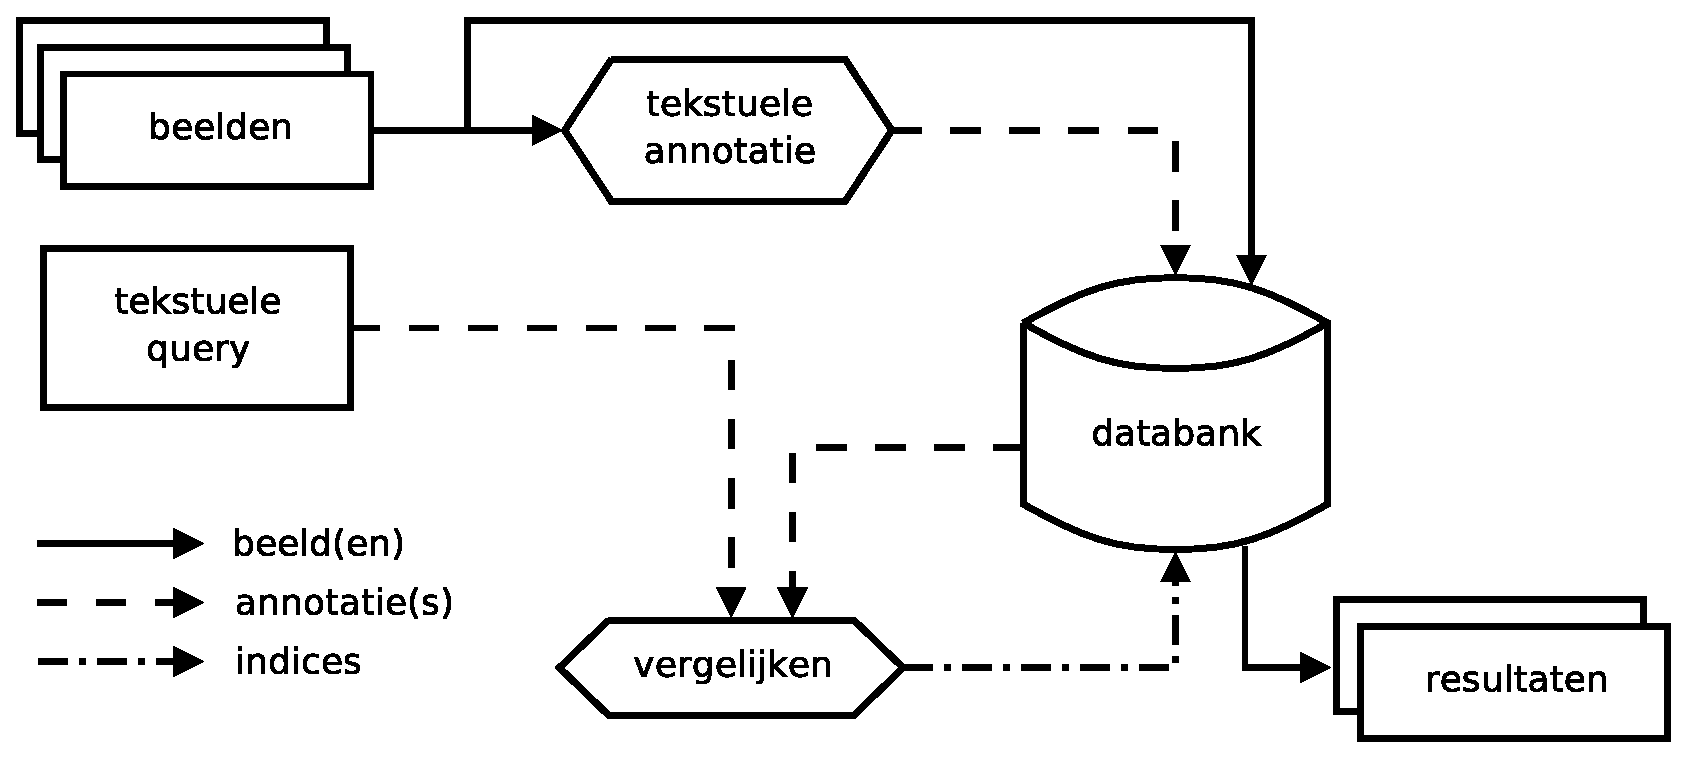
\includegraphics[width=10cm]{images/tbir.eps}
%\label{fig:tbir}
%}
%\subfigure[]{
%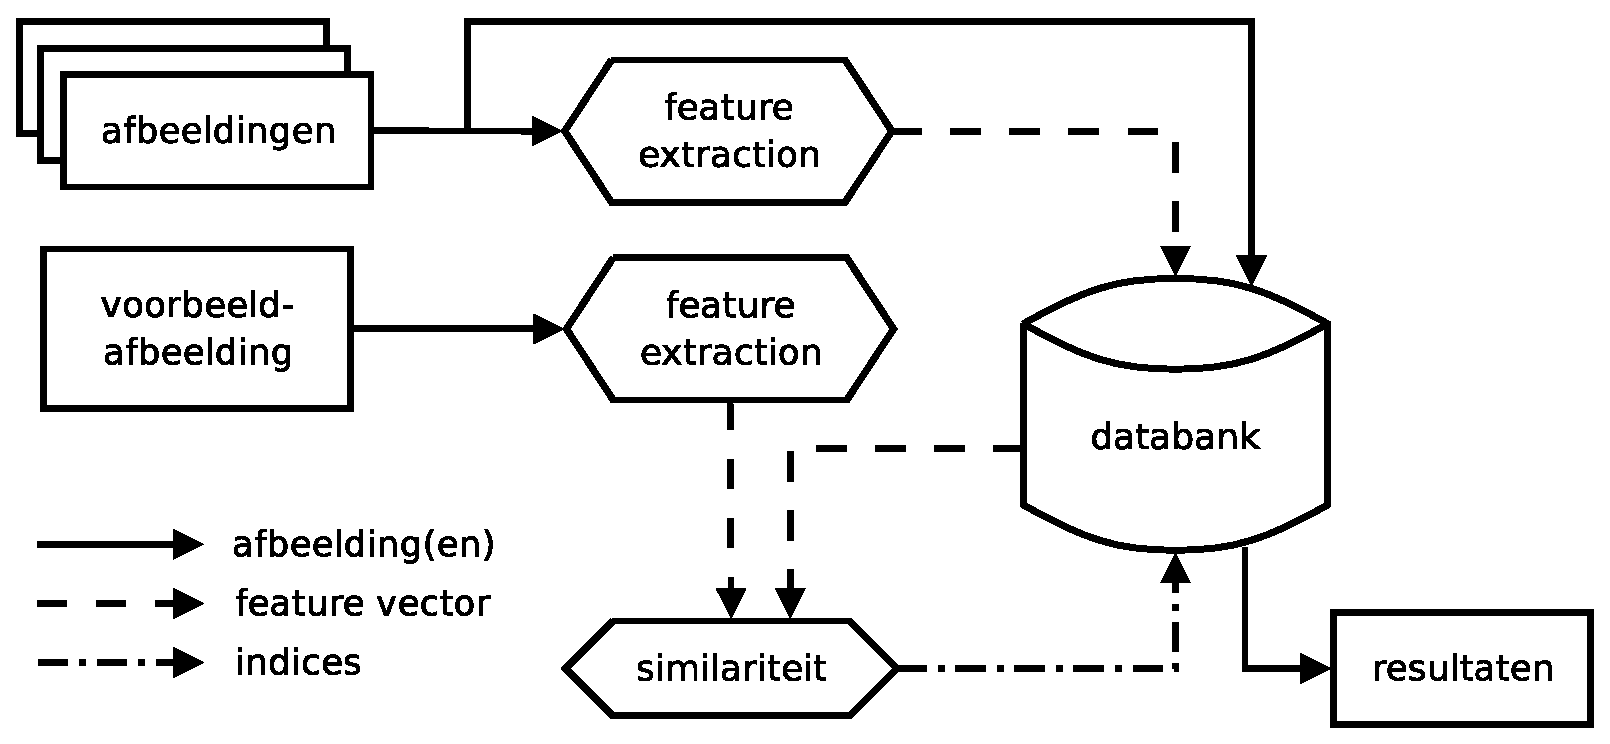
\includegraphics[width=10cm]{images/cbir.eps}
%\label{fig:cbir}
%}
\begin{tabular}{cccccc}

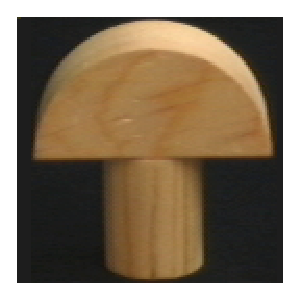
\includegraphics[width=2cm]{coil/beeld-0.eps} &
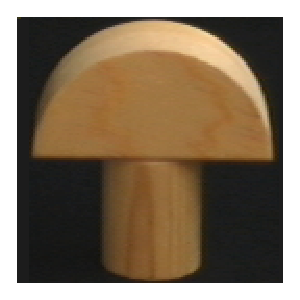
\includegraphics[width=2cm]{coil/beeld-1.eps} &
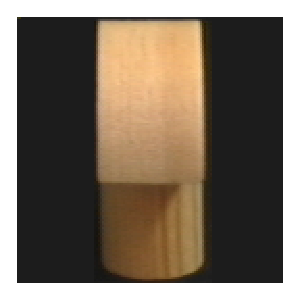
\includegraphics[width=2cm]{coil/beeld-2.eps} &
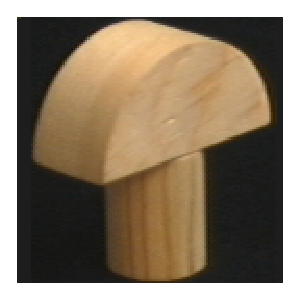
\includegraphics[width=2cm]{coil/beeld-3.eps} &
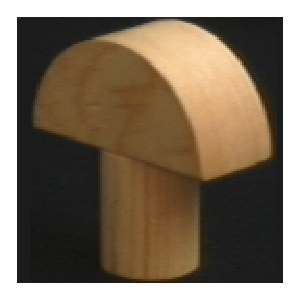
\includegraphics[width=2cm]{coil/beeld-4.eps} &
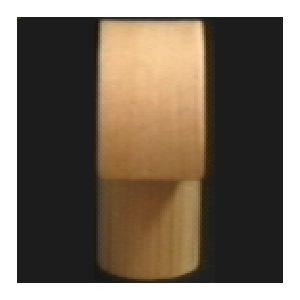
\includegraphics[width=2cm]{coil/beeld-5.eps} \\

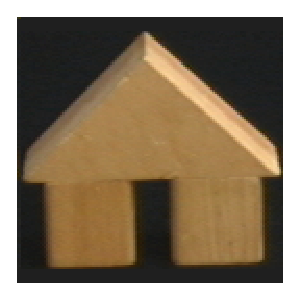
\includegraphics[width=2cm]{coil/beeld-42.eps} &
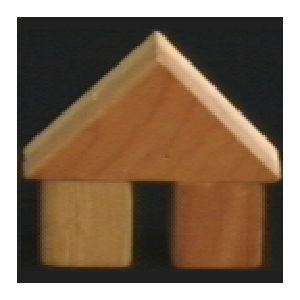
\includegraphics[width=2cm]{coil/beeld-43.eps} &
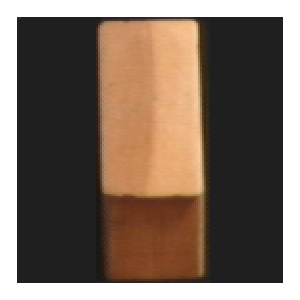
\includegraphics[width=2cm]{coil/beeld-44.eps} &
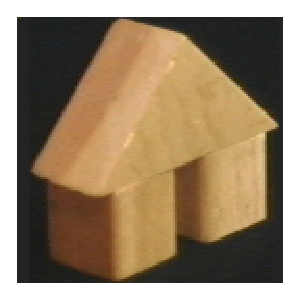
\includegraphics[width=2cm]{coil/beeld-45.eps} &
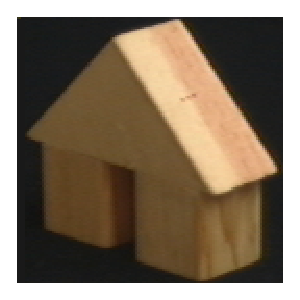
\includegraphics[width=2cm]{coil/beeld-46.eps} &
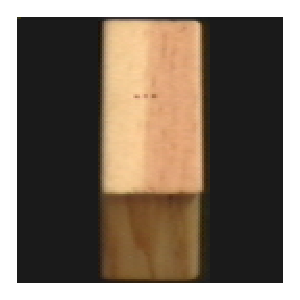
\includegraphics[width=2cm]{coil/beeld-47.eps} \\

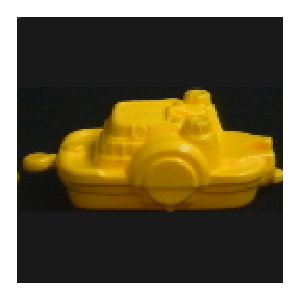
\includegraphics[width=2cm]{coil/beeld-12.eps} &
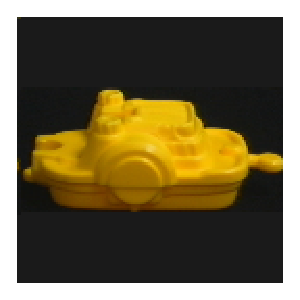
\includegraphics[width=2cm]{coil/beeld-13.eps} &
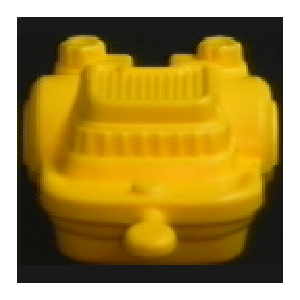
\includegraphics[width=2cm]{coil/beeld-14.eps} &
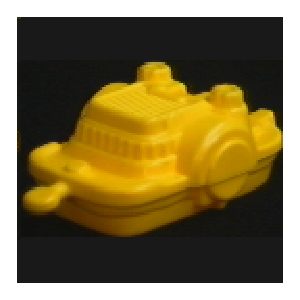
\includegraphics[width=2cm]{coil/beeld-15.eps} &
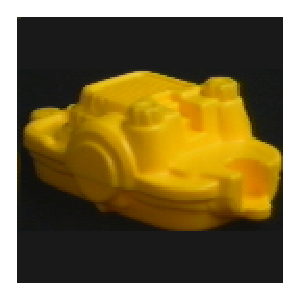
\includegraphics[width=2cm]{coil/beeld-16.eps} &
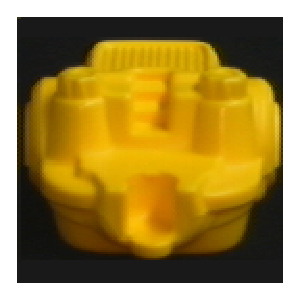
\includegraphics[width=2cm]{coil/beeld-17.eps} \\

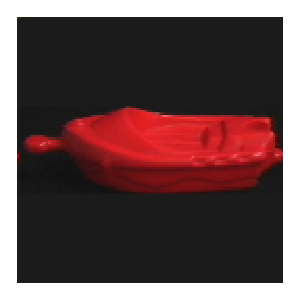
\includegraphics[width=2cm]{coil/beeld-18.eps} &
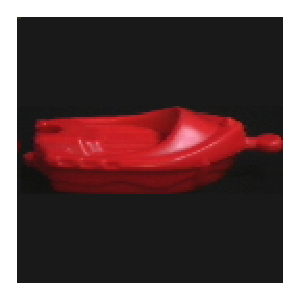
\includegraphics[width=2cm]{coil/beeld-19.eps} &
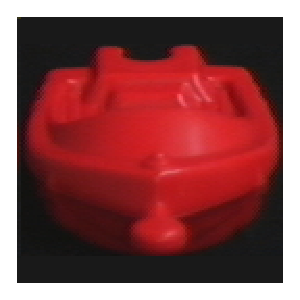
\includegraphics[width=2cm]{coil/beeld-20.eps} &
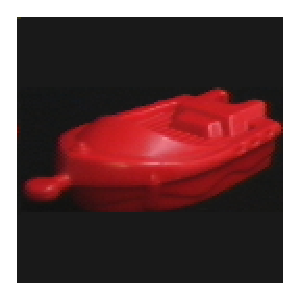
\includegraphics[width=2cm]{coil/beeld-21.eps} &
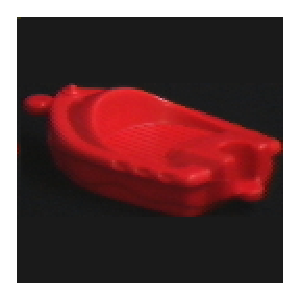
\includegraphics[width=2cm]{coil/beeld-22.eps} &
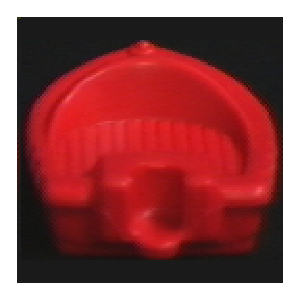
\includegraphics[width=2cm]{coil/beeld-23.eps} \\

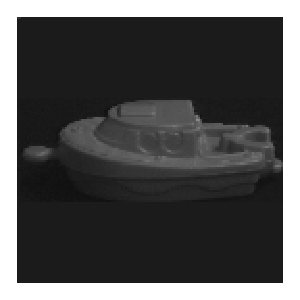
\includegraphics[width=2cm]{coil/beeld-24.eps} &
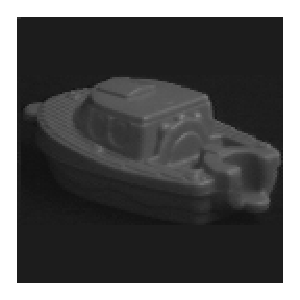
\includegraphics[width=2cm]{coil/beeld-25.eps} &
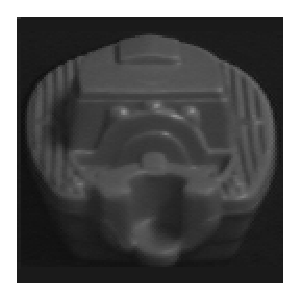
\includegraphics[width=2cm]{coil/beeld-26.eps} &
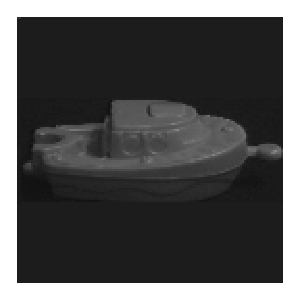
\includegraphics[width=2cm]{coil/beeld-27.eps} &
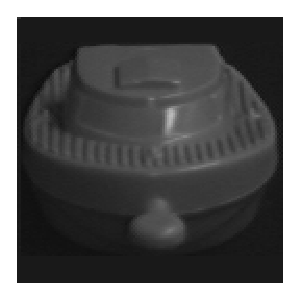
\includegraphics[width=2cm]{coil/beeld-28.eps} &
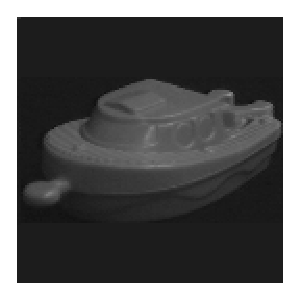
\includegraphics[width=2cm]{coil/beeld-29.eps} \\

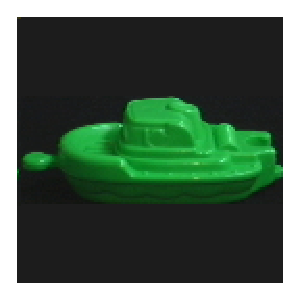
\includegraphics[width=2cm]{coil/beeld-54.eps} &
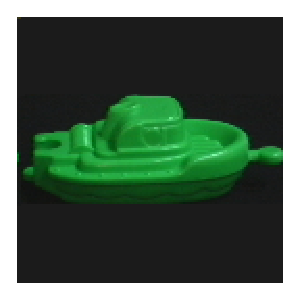
\includegraphics[width=2cm]{coil/beeld-55.eps} &
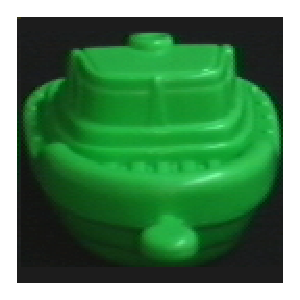
\includegraphics[width=2cm]{coil/beeld-56.eps} &
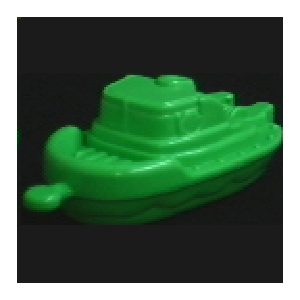
\includegraphics[width=2cm]{coil/beeld-57.eps} &
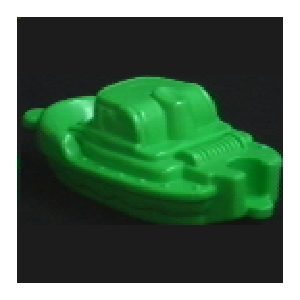
\includegraphics[width=2cm]{coil/beeld-58.eps} &
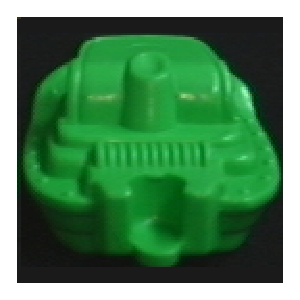
\includegraphics[width=2cm]{coil/beeld-59.eps} \\

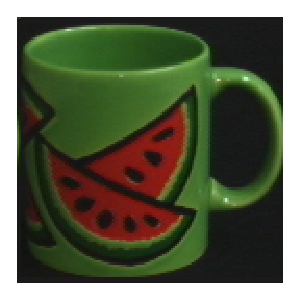
\includegraphics[width=2cm]{coil/beeld-30.eps} &
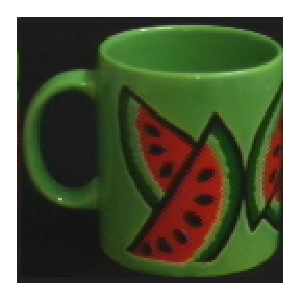
\includegraphics[width=2cm]{coil/beeld-31.eps} &
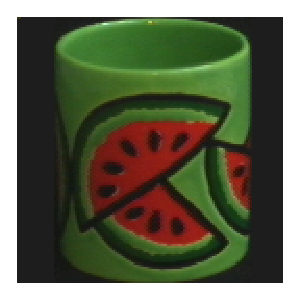
\includegraphics[width=2cm]{coil/beeld-32.eps} &
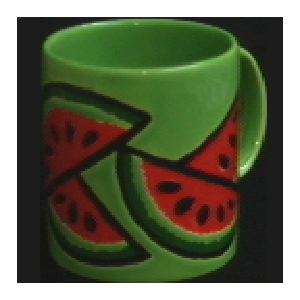
\includegraphics[width=2cm]{coil/beeld-33.eps} &
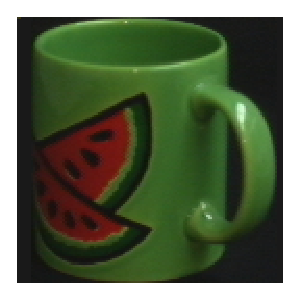
\includegraphics[width=2cm]{coil/beeld-34.eps} &
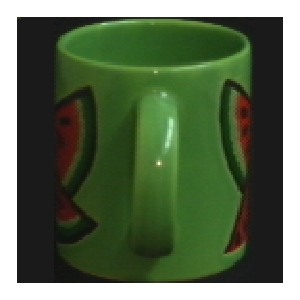
\includegraphics[width=2cm]{coil/beeld-35.eps} \\

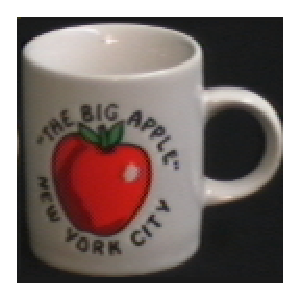
\includegraphics[width=2cm]{coil/beeld-36.eps} &
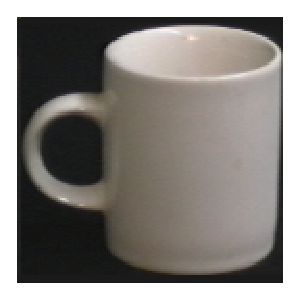
\includegraphics[width=2cm]{coil/beeld-37.eps} &
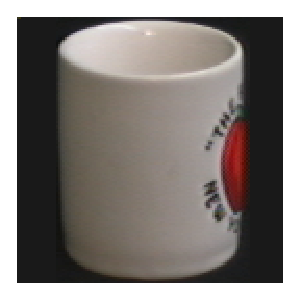
\includegraphics[width=2cm]{coil/beeld-38.eps} &
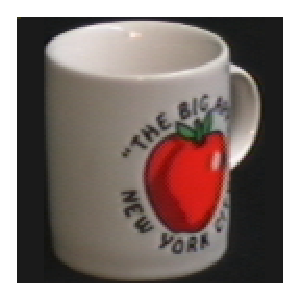
\includegraphics[width=2cm]{coil/beeld-39.eps} &
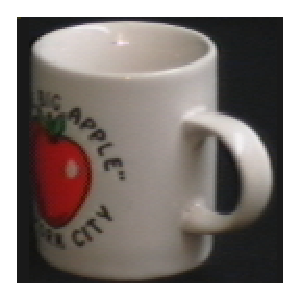
\includegraphics[width=2cm]{coil/beeld-40.eps} &
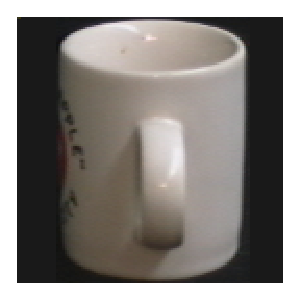
\includegraphics[width=2cm]{coil/beeld-41.eps} \\

\includegraphics[width=2cm]{coil/beeld-6.eps} &
\includegraphics[width=2cm]{coil/beeld-7.eps} &
\includegraphics[width=2cm]{coil/beeld-8.eps} &
\includegraphics[width=2cm]{coil/beeld-9.eps} &
\includegraphics[width=2cm]{coil/beeld-10.eps} &
\includegraphics[width=2cm]{coil/beeld-11.eps} \\

\includegraphics[width=2cm]{coil/beeld-48.eps} &
\includegraphics[width=2cm]{coil/beeld-49.eps} &
\includegraphics[width=2cm]{coil/beeld-50.eps} &
\includegraphics[width=2cm]{coil/beeld-51.eps} &
\includegraphics[width=2cm]{coil/beeld-52.eps} &
\includegraphics[width=2cm]{coil/beeld-53.eps} \\

\includegraphics[width=2cm]{coil/beeld-60.eps} &
\includegraphics[width=2cm]{coil/beeld-61.eps} &
\includegraphics[width=2cm]{coil/beeld-62.eps} &
\includegraphics[width=2cm]{coil/beeld-63.eps} &
\includegraphics[width=2cm]{coil/beeld-64.eps} &
\includegraphics[width=2cm]{coil/beeld-65.eps} \\

\end{tabular}
\caption{\label{fig:testcollectie}De gebruikte collectie van afbeeldingen.}
\end{center}
\end{figure}

Figuur~\ref{fig:testcollectie} bevat de collectie van afbeeldingen die we gaan 
gebruiken. Deze collectie bestaat uit een selectie van beelden uit
de \emph{Columbia object image library} \cite{coil-100}. Deze bibliotheek van afbeeldingen 
werd gegenereerd 
door een aantal roterende objecten op bepaalde vaste momenten te fotograferen. 
Onze testcollectie bestaat uit foto's van elf objecten. Van elke object zijn
er zes momentopnames, wat een totaal van $11 \times 6 = 66$ afbeeldingen geeft.

Voor het beoordelen van een rangschikking, gebruiken we de \emph{genormaliseerde gemiddelde rang} 
(GGR) \cite{muller:perf_eval}. Deze performantiemaat wordt toegepast op een collectie
van $N$ afbeeldingen. Voor elk van deze afbeeldingen bevat de collectie
$N_R$ zogenaamde \emph{relevante afbeeldingen}. In het geval van onze testcollectie geldt $N = 66$.
We gaan er in deze collectie vanuit dat foto's van eenzelfde object relevant zijn ten opzichte
van elkaar: $N_R = 6$. Beschouw nu de vector 
$(r_1,r_2,\ldots,r_{N_R}) \in \{1,2,\ldots,N\}^{N_R}$, waarbij $r_i$ het
rangnummer van de $i$-de relevante afbeelding voorstelt. De performantiemaat
wordt dan als volgt gedefinieerd:
\begin{definitie}
De genormaliseerde gemiddelde rang wordt gegeven door de volgende afbeelding:
$$
\begin{array}{llll}
\textrm{GGR}: 	& \{1,2,\ldots,N\}^{N_R} & \to 	& [0,1] \\
		& (r_1,r_2,\ldots,r_{N_R}) & \mapsto &
	{\displaystyle\frac{1}{N N_R}\left(\left(\sum_{i=1}^{N_R}r_i\right) - \frac{N_R (N_R + 1)}{2}\right)},\\ 
	& & & \qquad \forall (r_1, r_2, ..., r_{N_R}) \in \{1,2,\ldots,N\}^{N_R}
\end{array}
$$
\end{definitie}
\noindent
Deze maat nadert naar 1 naarmate de performantie slechter wordt.

Tot nu toe hebben we er echter nog geen rekening mee gehouden dat de performantie van
een similariteitsmaat afhankelijk kan zijn van de gekozen voorbeeld-afbeelding. Dit probleem lossen we
op door de GGR te berekenen voor meerdere voorbeelden en het gemiddelde van de bekomen waarden
te beschouwen. We kiezen hierbij de beelden uit de linker kolom van 
figuur~\ref{fig:testcollectie} als voorbeeld-afbeeldingen. De waarde die we zo bekomen noemen we de
\emph{globale genormaliseerde gemiddelde rang} (GGGR). Het is deze waarde die we zullen gebruiken
om de performantie van een similariteitsmaat te evalueren. We zullen dus met andere woorden op
zoek gaan naar similariteitsmaten waarvan de GGGR zo klein mogelijk is.


\section{Pixel-gebaseerd}

\subsection{Grijswaardebeelden}

\subsubsection{Representatie}

Een \emph{binair beeld} is een beeld dat enkel witte en zwarte beeldpunten bevat. We kunnen een 
$n$-dimentionaal binair beeld dus modelleren als een scherpe verzameling $A$ in $\mathbb{R}^n$, met:
$$
\begin{array}{rcl}
x \in A & \iff & x \textrm{ is een wit punt in het beeld} \\
x \notin A & \iff & x \textrm{ is een zwart punt in het beeld}
\end{array}
$$ 
In de praktijk wordt een binair beeld echter voorgesteld als een rooster bestaande uit een
eindig aantal beeldpunten. Men kiest dus eerder $\mathbb{N}^2$ als universum.

Behalve wit en zwart, kan een \emph{grijswaardebeeld} ook grijstinten bevatten. Deze grijstinten
kunnen voorgesteld worden aan de hand van waarden uit het open eenheidsinterval $]0,1[$, waarbij
geldt: hoe groter de grijswaarde, hoe lichter de grijstint. Een $n$-dimensionaal grijswaardebeeld
kan dus gemodelleerd worden als een vaagverzameling $A$ in $\mathbb{R}^n$ bepaald door:
$$
\begin{array}{rcl}
A(x) = 1 & \iff & x \textrm{ is een wit punt in het beeld} \\
A(x) = 0 & \iff & x \textrm{ is een zwart punt in het beeld} \\
A(x) \in\ ]0,1[ & \iff & x \textrm{ is een beeldpunt met een grijstint}
\end{array}
$$
Ook bij grijswaardebeelden is het universum in de praktijk eerder $\mathbb{N}^2$.

\subsubsection{Similariteitsmaten}

Door de bovenstaande representatie te combineren met de vaagsimilariteitsmaten uit 
\ref{sectie:vaagsimilariteitsmaten}, bekomen we 23 similariteitsmaten. Deze maten
vergelijken beide afbeeldingen door elk van hun beeldpunten met elkaar te vergelijken.
Deze beeldpunten worden ook \emph{picture elements} of kortweg \emph{pixels} genoemd. Vandaar
dat we zeggen dat deze similariteitsmaten \emph{pixel-gebaseerd} zijn.

Men noemt het aantal pixels in een afbeelding de \emph{resolutie} van die afbeelding. Het is
duidelijk dat deze pixel-gebaseerde maten vereisen dat beide afbeeldingen dezelfde resolutie 
hebben. Bovendien kunnen ze enkel gebruikt worden om grijswaardebeelden te vergelijken.


\subsection{Kleurbeelden}

\subsubsection{Kleurruimten}

Een \emph{kleurmodel} is een abstract mathematisch model dat beschrijft hoe kleuren gerepresenteerd 
kunnen worden als $n$-tallen. RGB is het meest gebruikte kleurmodel. In dit model is elke kleur
een gewogen som van drie hoofdkleuren: rood, groen en blauw. De gewichten van deze som
worden gebruikt als componenten van het drietal dat deze kleur voorstelt. Naast RGB zijn ook
HSV en L*a*b* populaire kleurmodellen.

De kleuren die men op basis van een bepaald model kan voorstellen vormen een \emph{kleurruimte}. 
In het geval van RGB is dit een driedimentionale ruimte. De kleuren in deze ruimte zijn afhankelijk
van de manier waarop men ``rood'', ``groen'' en ``geel'' definieert. Veelgebruikte kleurenruimtes 
op basis van het RGB model zijn sRGB en Adobe RGB.

Hoewel het strikt gezien niet correct is, gebruikt men de term ``kleurruimte'' vaak ook voor het
kleurmodel. Men heeft het dus vaak over \emph{de} RGB kleurruimte, terwijl er eigenlijk meerdere
kleurruimtes bestaan die gebaseerd zijn op RGB. 

\subsubsection{Representatie}

Bij een \emph{kleurbeeld} heeft elke pixel een bepaalde kleur. Deze kleur wordt beschreven met
behulp van een kleurmodel. Ze wordt bijgevolg voorgesteld als een $n$-tal uit
$\mathbb{R}^n$. Dergelijke $n$-tallen kunnen we normaliseren tot $n$-tallen uit $[0,1]^n$. 
Dit laat ons toe om een $m$-dimensionaal kleurbeeld te modelleren als een L-vaagverzameling in 
$\mathbb{R}^m$, waarbij $L=[0,1]^n$.

We hebben reeds vermeld dat de similariteitsmaten uit \ref{sectie:vaagsimilariteitsmaten}
uitbreidbaar zijn naar L-vaag\-ver\-za\-me\-ling\-en. Zoals in \ldots beperken we ons tot het 
RGB model en veralgemenen we de be\-wer\-king\-en waarvan de similariteitsmaten gebruik maken 
als volgt naar kleuren in dit model:
$$
\begin{array}{rcl}
|c| & = & \frac{1}{\sqrt{3}} \cdot \sqrt{r^2 + g^2 + b^2} \\[5pt]
c - c' & = & (r-r',g-g',b-b') \\[5pt]
1 - c & = & (1,1,1) - c \\[5pt]
\min (c,c') & = & c \quad\textrm{als } c \leq_{RGB} c' \\
		  & = & c' \quad\textrm{anders} \\[5pt]
\max (c,c') & = & c' \quad\textrm{als } c \leq_{RGB} c' \\
		  & = & c \quad\textrm{anders}
\end{array}
$$
met $c(r,g,b)$ en $c'(r',g',b')$ kleuren uit $[0,1]^3$ en $\leq_{RGB}$ de ordening voor
kleuren in het RGB model uit \ldots. Deze ordening wordt als volgt gedefinieerd:
$$
\begin{array}{rcl}
c <_{RGB} c' & \iff & d(c,Bl) < d(c',Bl)\ \lor \\
			   &	  & \quad(d(c,Bl) = d(c',Bl) \land d(c,Wh) > d(c',Wh)) \\[5pt]
c >_{RGB} c' & \iff & d(c,Wh) < d(c',Wh)\ \lor \\
			   &	  & \quad(d(c,Wh) = d(c',Wh) \land d(c,Bl) > d(c',Bl)) \\[5pt]
c =_{RGB} c'   & \iff & (d(c,Bl) = d(c',Bl) \land d(c,Wh) = d(c',Wh))
\end{array}
$$
waarbij $Bl=(0,0,0)$, $Wh=(1,1,1)$ en $d$ de Euclidische afstand.

\section{Kleur-gebaseerd}
